%vim: spelllang=uk
\documentclass[simple,14pt,utf8,ukrainian]{eskdtext}
\usepackage{eskddstu}
\ESKDtitle{{\small Мінімізація витрат на побудову огороджень}}
\ESKDdocName{Пояснювальна записка.}
\ESKDsignature{ІАЛЦ.468800.001 ПЗ}
\ESKDauthor{Погода~М.\,В.}
\ESKDchecker{Олефір~О.\,С.}
\ESKDgroup{{\scriptsize НТУУ ,,КПІ'', ФПМ, КМ-92}}
\ESKDapprovedBy{{\scriptsize Молчанов~О.\,А.}}
\renewcommand{\ESKDfontShape}{\upshape}

\usepackage{pdflscape}
\usepackage{cmap} % чтобы работал поиск по PDF
\usepackage[utf8]{inputenc}
%\usepackage[english,ukrainian]{babel}
\usepackage[T2A]{fontenc}
\usepackage{indentfirst}
\usepackage{concrete}

%\usepackage{textcase}
%\usepackage[pdftex]{graphicx}

\pdfcompresslevel=9 % сжимать PDF
%\usepackage{pdflscape} % для возможности альбомного размещения некоторых страниц
%\usepackage[pdftex,unicode]{hyperref}
% настройка ссылок в оглавлении для pdf формата
%\hypersetup{unicode=true
           %,pdftitle={Пояснювальна записка}
           %,pdfauthor={Погода Михайло}
           %,pdfcreator={pdflatex}
           %,pdfsubject={}
           %,pdfborder={0 0 0}
           %,bookmarksopen
           %,bookmarksnumbered
           %,bookmarksopenlevel=2
           %,pdfkeywords={}
           %,colorlinks=true % установка цвета ссылок в оглавлении
           %,citecolor=black
           %,filecolor=black
           %,linkcolor=black
           %,urlcolor=blue
           %}

\usepackage{listings}
\lstloadlanguages{C++}
\lstset{language=C++,basicstyle=\scriptsize,frame=tb,commentstyle=\itshape,stringstyle=\bfseries,extendedchars=false}
\usepackage{amsmath}
\usepackage{amssymb}

\begin{document}
\ESKDthisStyle{empty}
\begin{titlepage}
    \begin{center}
        \MakeUppercase{Міністерство освіти і науки України}

        Національний технічний університет України

        ,,Київський політехнічний інститут''

        \vspace*{0.5cm}

        Факультет прикладної математики

        \vfill

        \textbf{\MakeUppercase{Курсовий проект}}

        з дисципліни:

        ,,Програмне забезпечення ЕОМ''

        \textbf{Мінімізація витрат матеріалів на побудову огороджень.\\
          Алгорітм Грехема}
    \end{center}

    \vfill

    \begin{minipage}{0.15\textwidth}
      Виконав:

      Керівник:
    \end{minipage}
    \begin{minipage}{0.3\textwidth}
      студент групи КМ-92

      к.\,т.\,н., доцент
    \end{minipage}
    \begin{minipage}{0.2\textwidth}
      Погода~М.\,В.

      Олефір~О.\,С.
    \end{minipage}
    \begin{minipage}{0.20\textwidth}
      \underline{\hspace{0.8\textwidth}}

      \underline{\hspace{0.8\textwidth}}
    \end{minipage}

    \vfill

    \vfill

    \begin{center}
        Київ --- 2013
    \end{center}
\end{titlepage}
\ESKDthisStyle{formII}
\tableofcontents
\newpage

\section*{ВСТУП}
\addcontentsline{toc}{section}{ВСТУП}
  Сьогодні, під час початкового проектування майбутньої будівлі, часто виникає
  задача огородження будівельного майданчика.

  Майданчик потрібно огородити так, щоб на цей майданчик мали доступ лише
  будівники.
  Сам матеріал огорожі обирається найдешевшим із можливих варіантів, тому
  на цьому етапі оптимальна форма забору не має суттєвого значення.

  Після будівництва огорожу скоріш за все замінять на більш
  естетично"=приємнішу огорожу, а отже її ціна буде значно вищою.
  У цьому випадку було б гарно спроектувати огорожу найоптимальнішим способом,
  так, щоб загальна її довжина була мінімальною.

  Найпростішим способом є спорудження огорожі у формі такого прямокутника,
  який би містив усі точки території.
  Але цей метод не дозволяє отримати оптимальну форму огорожі.

  Для територій складних форм кращим засобом оперативного вирішення цієї
  задачі є використання спеціалізованого комп’ютерного забезпечення на базі
  сучасних математичних методів оптимізації.

  Розроблене програмне забезпечення призначене для пошуку найоптимальніший
  форми огорожі за допомогою сучасного алгоритму, та не вимагає від
  користувача спеціальної математичної підготовки.
\newpage

\section{\MakeUppercase{Технічне завдання}}
  \subsection*{Назва розробки}
    ,,Мінімізація витрат матеріалів на побудову заборів''.
  \subsection*{Галузь застосування}
    Завдяки оптимізації форми забору можливо значно скоротити витрати
    матеріалів на його побудову.

  \subsection*{Підстави для розробки}
    Підставою для розроблення є навчальний план підготовки бакалавра за
    напрямом 6.040301 ,,Прикладна математика'' та навчальна програма
    дисципліни ,,Програмне забезпечення ЕОМ''.

  \subsection*{Призначення розробки}
    Метою є створення програмного забезпечення, за допомогою якого можна
    знайти оптимальну форму забору навколо зазначеної території, таку, що
    витрати матеріалу на її побудову були б мінімальними.

    У функціонал програми входить: введення координат території, що повинна
    бути огородженої; знаходження оптимальної форми огородження; відображення
    моделі на екрані; обчислення довжини отриманого огородження.

  \subsection*{Вимоги до програмного виробу}
    \subsubsection*{Вимоги до функціональних характеристик}
        Програмне забезпечення, що розробляється, повинно виконувати такі
        функції та задовольняти таким вимогам:
        \begin{itemize}
            \item можливість введення користувачем даних;
            \item обчислення оптимальної форми огородження та його довжини;
            \item можливість виведення отриманих результатів на екран.
        \end{itemize}

    \subsubsection*{Вимоги до умов експлуатації}
        Дане програмне забезпечення буде одного разу під час проектування
        огорожі для території.

    \subsubsection*{Вимоги до складу й параметрів технічних засобів}
        Вимоги до персонального комп’ютера, на якому буде використовуватись
        розроблене програмне забезпечення:
        \begin{itemize}
            \item Intel Pentium 166 MHz або вище
            \item 128 Мб ОЗУ
            \item 10 Мб вільного місця на диску;
            \item VGA або вища роздільна здатність монітора (для подальшої
                роботи з графікою);
            \item клавіатура, миша.
        \end{itemize}
    \subsubsection*{Вимоги до інформаційної та програмної сумісності}
        Розроблюване програмне забезпечення повинно працювати під керування
        операційної системи Windows XP/7 або GNU/Linux.

  \subsection*{Техно"=економічні показники}
    Програмних засобів, що б були призначені для цієї задачі, не було
    знайдено.

  \subsection*{Стадії і етапи розробки}

    \begin{tabular}[t]{|p{1em}|p{23em}|p{5em}|}
        \hline
        \No & Назва роботи & Термін виконання\\
        \hline
        1 & Вибір теми & 20.09.12 \\
        \hline
        2 & Огляд літератури. Вивчення математичних методів розв’язування
        задач & 04.10.12 \\
        \hline
        3 & Вибір, обґрунтування, освоєння методу розв’язування задачі.
        Розв’язування контрольних прикладів & 18.10.12 \\
        \hline
        4 & Проектування архітектури розроблюваних програмних засобів &
        25.10.12 \\
        \hline
        5 & Визначення складу та формату вхідних даних та результатів кожної
        програми & 01.11.12 \\
        \hline
        6 & Розробка алгоритму & 15.11.12 \\
        \hline
        7 & Розробка мови управління програмою & 22.11.12 \\
        \hline
        8 & Програмна реалізація & 06.12.12 \\
        \hline
        9 & Оформлення РГР & 13.12.12 \\
        \hline
        10 & Уточнення технічного завдання & 14.02.13 \\
        \hline
        11 & Налагодження програм та експериментальні розрахунки & 21.02.13 \\
        \hline
        12 & Розв'язок контрольних задач на ЕОМ & 7.03.13 \\
        \hline
        13 & Оформлення пояснювальної записки & 14.03.13 \\
        \hline
        14 & Випробування розроблених програм в присутності викладача &
        21.03.13 \\
        \hline
        15 & Захист курсової роботи перед комісією & 28.03.13 \\
        \hline
    \end{tabular}

  \subsection*{Порядок контролю і здачі}
    Вірність результатів розробленого програмного забезпечення перевіряється
    на виконанні контрольних прикладів та задачах, запропонованих комісією.

    Розроблене програмне забезпечення представляється комісії для оцінювання.
\newpage
\section{ПОСТАНОВКА ЗАДАЧІ}
    \subsection*{Вимоги до функціональних характеристик}
        Програмне забезпечення, що розробляється, повинно виконувати такі
        функції та задовольняти таким вимогам:
        \begin{itemize}
            \item можливість введення користувачем даних;
            \item обчислення оптимальної форми огородження та його довжини;
            \item можливість виведення отриманих результатів на екран.
        \end{itemize}

    \subsection*{Вимоги до складу й параметрів технічних засобів}
        Вимоги до персонального комп’ютера, на якому буде використовуватись
        розроблене програмне забезпечення:
        \begin{itemize}
            \item Intel Pentium 166 MHz або вище
            \item 128 Мб ОЗУ
            \item 10 Мб вільного місця на диску;
            \item VGA або вища роздільна здатність монітора (для подальшої
                роботи з графікою);
            \item клавіатура, миша.
        \end{itemize}
    \subsection*{Вимоги до надійності та до сервісних засобів, обслуговуючих
    програму}
      \begin{itemize}
        \item Алгоритм програми має передбачувати обробку всіх можливих
          виключних ситуацій з метою запобігання виникнення системних
          переривань.
        \item Програма повинна мати зручне меню користувача, яке дозволить
          швидко освоїти усі можливості системи.
        \item Система повинна працювати чітко, і надавати користувачеві
          виключно правдиву інформацію (з цією метою система виконає завдання
          контрольних прикладів, які мають розв’язок без використання ЕОМ).
      \end{itemize}

\section{ПРОЕКТУВАННЯ ПРОГРАМНИХ ЗАСОБІВ}
  Як показали дослідження, мінімальну довжину має огорожа в формі випуклої
  оболонки, що була побудована для усіх точок території, котру потрібно
  огородити.\cite{book1}

  \emph{Випуклою оболонкою} множини $\mathbb{X}$ називають найменшу випуклу
  множину, що містить $\mathbb{X}$.
  ,,Найменша множина'' тут означає найменший елемент по відношенню до
  вкладання множин, тобто така випукла множина, що містить цю фігуру, що
  міститься в будь"=якій іншій випуклій множини, що містить цю фігуру.\cite{book2}

  Множину в афінному просторі називають \emph{випуклою} якщо вона містить
  разом з будь"=якими двома точками й відрізок, що їх з’єднує

  \subsection{Огляд можливих методів розв’язку}
    Існує декілька методів (алгоритмів), що дозволяють побудувати випуклу
    оболонку для множини точок.
    \begin{itemize}
      \item \emph{Алгоритм Грехема}.
        В цьому алгоритмі задача про пошук випуклої оболонки вирішується за
        допомогою стека, створеного з точок"=кандидатів.
        Усі точки початкової множини заносяться в стек, а потім точки, що не
        належать до вершин випуклої оболонки видаляються з нього.
        По завершенні роботи алгоритму в стеці залишаються лише вершини
        оболонки в порядку їх обходу проти годинникової стрілки.\cite{book3}
    \item \emph{Алгоритм Джарвіса}.
      Алгоритм можна уявити як обтягування мотузкою множини вбитих у дошку
      цвяхів.
      Алгоритм працює за час \verb'O(nh)', де \verb'n' --- загальне число
      точок на площині, \verb'h' --- число точок у випуклій оболонці.\cite{book4}
    \item \emph{Алгоритм Чана}.
      Цей алгоритм є комбінацією двох більш повільних алгоритмів (сканування
      за Грехему й згортання за Джарвісом).
      Недоліком сканування за Грехемом є необхідність сортування усіх точок за
      полярним кутом, що може займати досить багато часу.
      Згортання за Джарвісом потребує перебору всіх точок для кожної з вершин
      випуклої оболонки, що в найгіршому випадку може тривати квадратичний
      час.\cite{book5}
    \item \emph{Алгоритм швидкої оболонки}.
      Використовує ідею швидкого сортування Хоара.
    \item \emph{Алгоритм Кіркпатрика}
  \end{itemize}
  \subsection{Опис обраного математичного методу}
    \emph{Алгоритм Грехема} --- алгоритм побудови випуклої оболонки в
    двовимірному просторі.
    В цьому алгоритмі задача про пошук випуклої оболонки вирішується за
    допомогою стека, створеного з точок"=кандидатів.
    Усі точки початкової множини заносяться в стек, а потім точки, що не
    належать до вершин випуклої оболонки видаляються з нього.
    По завершенні роботи алгоритму в стеці залишаються лише вершини
    оболонки в порядку їх обходу проти годинникової стрілки.

  \subsection{Опис контрольних прикладів}
  \label{ssec:ex}
    \point{Приклад №1}
    \[
      A = \left\{
        (0, 0), (1, 0), (2, 0),
        (0, 1), (1, 1), (2, 1),
        (0, 2), (1, 2), (2, 2)
      \right\}
    \]

    \[ \mathop{Conv} A = \left\{
        (0, 0), (2, 0), (2, 2), (0, 2)
       \right\}
    \]
    \point{Приклад №2}
    \[
      A = \left\{
        (0, 0), (1, 0), (2, 0),
        (0, 1), (1, 1),
        (0, 2)
      \right\}
    \]

    \[
      \mathop{Conv} A = \left\{
        (0, 0), (2, 0), (0, 2)
      \right\}
    \]
\newpage
\section{ПРОЕКТУВАННЯ ПРОГРАМНИХ ЗАСОБІВ}
\subsection{Архітектура програмного забезпечення}
    %\begin{figure}[h]
      %\caption{Схема взаємодії програм}
      %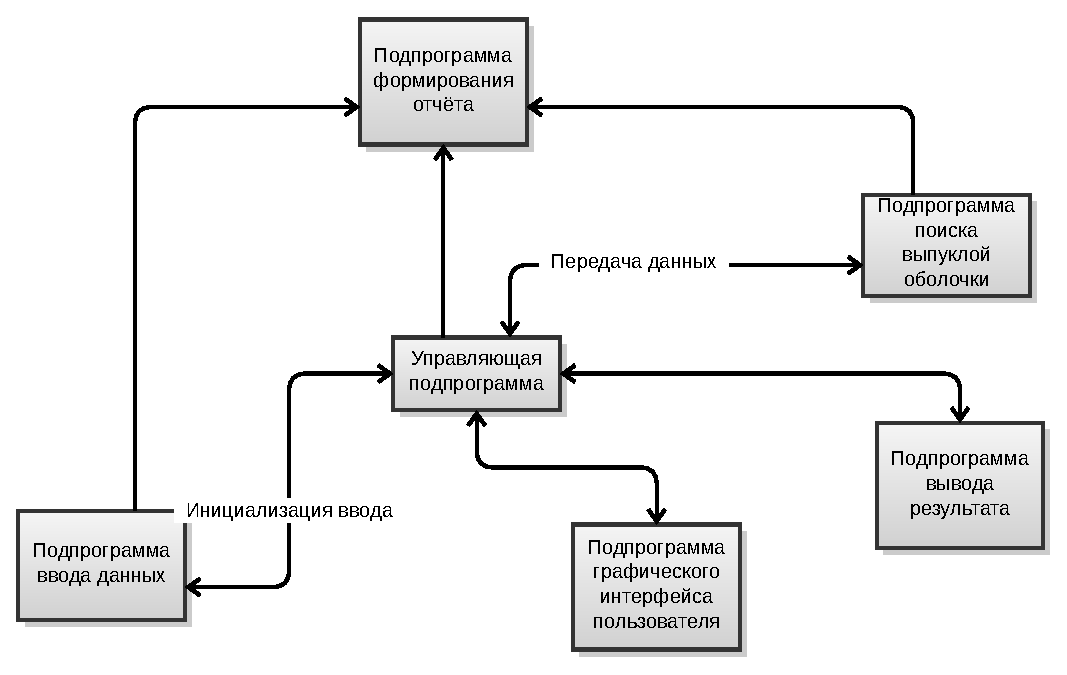
\includegraphics{scheme.eps}
    %\end{figure}

    Програмне забезпечення можна розділити на декілька підпрограм, кожна з
    яких виконує свою функцію.

    Весь процес рішення задачі можна представити як послідовність обміну
    інформацією між цими підпрограмами:
    \begin{enumerate}
      \item Підпрограма керування ініціює графічний інтерфейс і очікує дій
        користувача.
      \item Підпрограма керування отримує запит на ініціацію дій від
        графічного інтерфейсу.
      \item Підпрограма керування ініціює введення даних.
      \item Підпрограма керування пересилає вхідні дані підпрограмі пошуку
        випуклої оболонки й очікує результатів обчислень.
      \item Підпрограма керування ініціює виведення даних й графічне
        представлення результату.
      \item Підпрограма ведення звіту очікує сигналів від інших підпрограм.
    \end{enumerate}

    Між підпрограмами існують такі зв’язки:
    \begin{itemize}
      \item Керуюча підпрограма обробляє сигнали від інших підпрограм і
        передає їм своєчасні сигнали керування.
      \item Підпрограма введення отримує сигнал керування й дані, що були
        введені користувачем (множину точок або ім’я файлу, що містить таку
        множину), обробляє ці дані (розпізнає введені користувачем точки або
        зчитує дані з файлу) й передає керуючій підпрограмі множину точок у їх
        внутрішньому представленні.
      \item Підпрограма виведення отримує сигнал керування та дані, перетворює
        їх у належний вид (бінарний або текстовий) і виводить їх на потрібний
        пристрій вивдення.
      \item Підпрограма графічного інтерфейсу користувача отримує керуючі
        сигнали й різні дії користувача.
      \item Підпрограма ведення звіту отримує повідомлення про стан програми
        від інших підпрограм, та зберігає їх у формі звіту.
    \end{itemize}
  \subsection{Алгоритм роботи прикладного програмного забезпечення}
    \begin{figure}[h]
      \begin{center}
        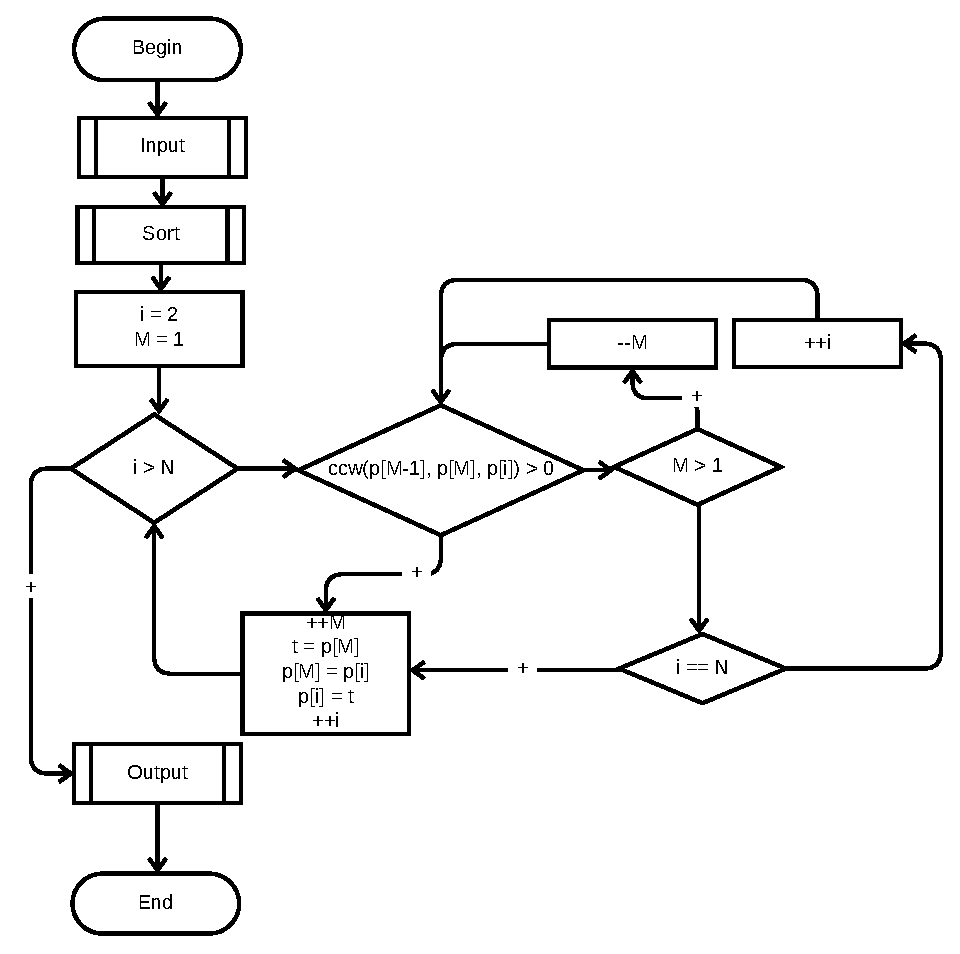
\includegraphics{algo.eps}
      \end{center}
      \caption{Блок"=схема роботи алгоритму}
      \label{fig:algo}
    \end{figure}

    \begin{figure}[h]
      \begin{center}
        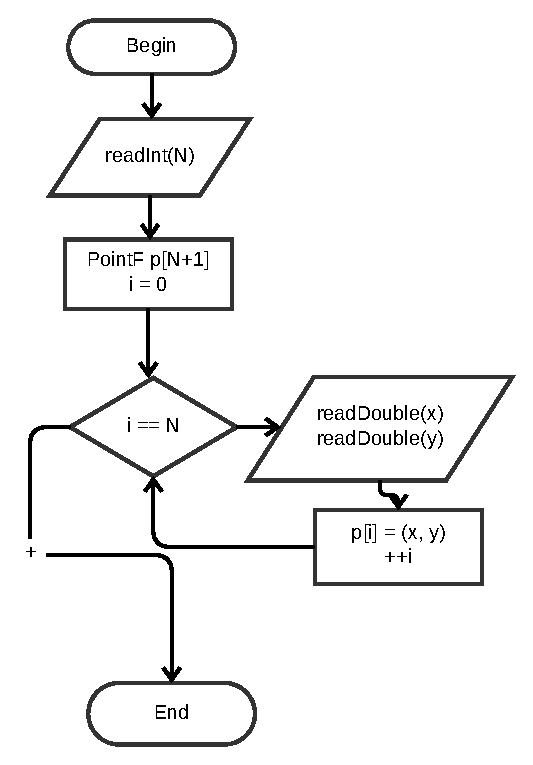
\includegraphics{input.eps}
      \end{center}
      \caption{Блок"=схема введення даних}
      \label{fig:input}
    \end{figure}

    \begin{figure}[h]
      \begin{center}
        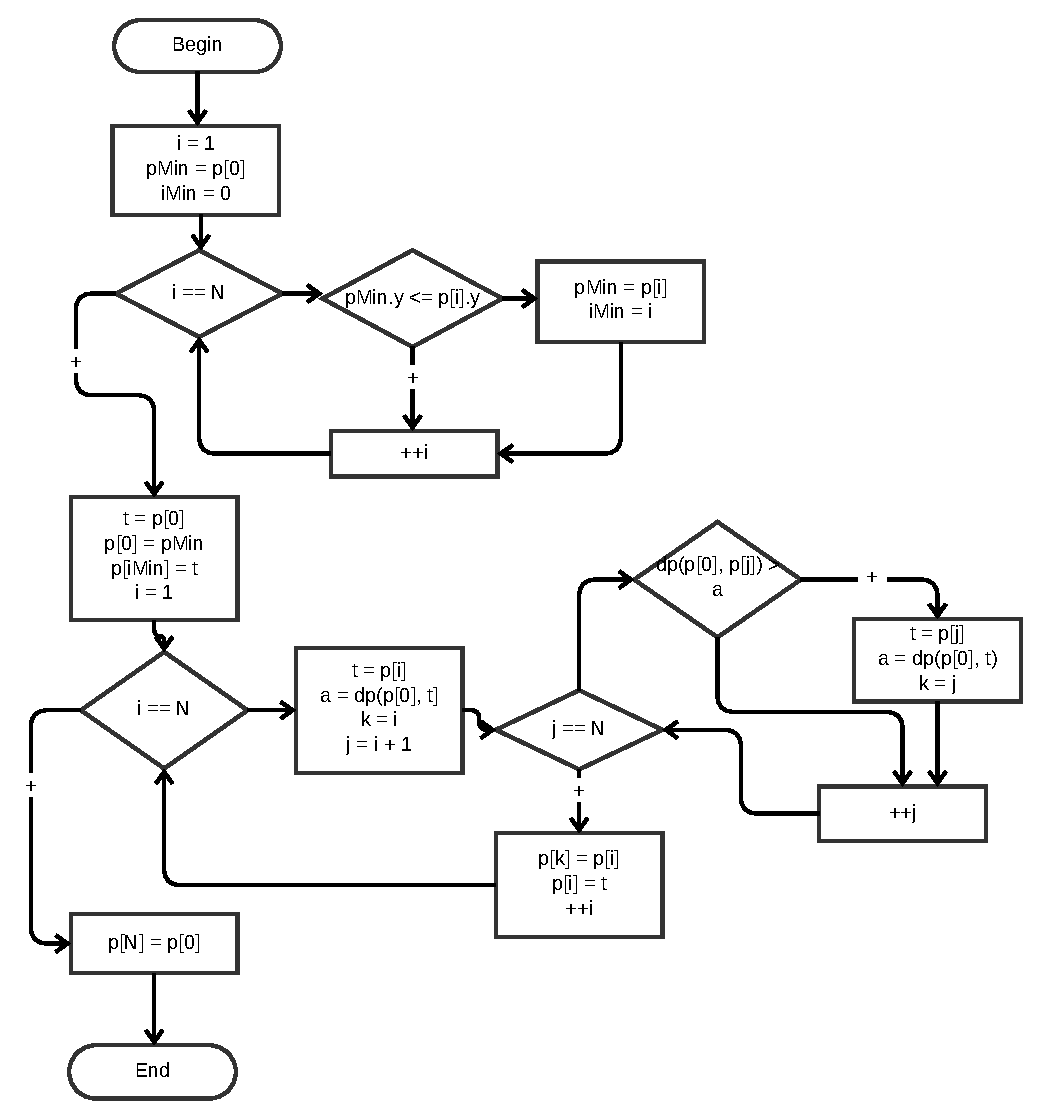
\includegraphics{sort.eps}
      \end{center}
      \caption{Блок"=схема підготування множини до роботи}
      \label{fig:sort}
    \end{figure}

    \begin{figure}[h]
      \begin{center}
        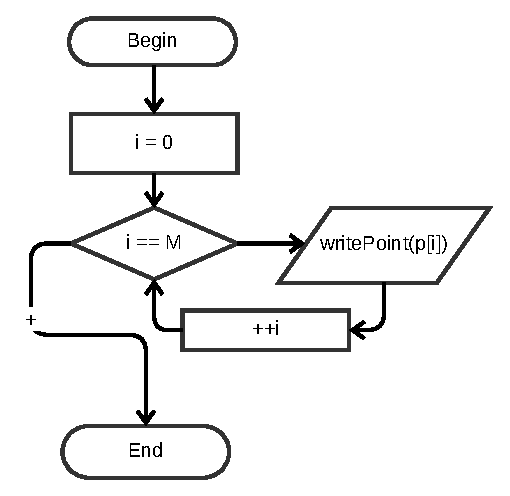
\includegraphics{output.eps}
      \end{center}
      \caption{Блок"=схема виведення результату}
      \label{fig:output}
    \end{figure}
    \clearpage
  \subsection{Формат вхідних даних і результатів роботи}
    Пошук випуклої оболонки на площині полягає в виборі з множини точок тільки
    тих точок, що є вершинами випуклої оболонки цієї множини.

    Таким чином,
    \begin{equation}
      \mathop{conv} A : \mathbb{R}^2 \rightarrow \mathbb{R}^2
      \label{eq:1}
    \end{equation}

    Для представлення точки на площини можна використовувати абстрактний тип
    даних, що зберігатиме її координати.

    Таким чином, програма отримує на вхід множину (масив, список, колекцію)
    пар дійсних чисел, й повертає в результаті свого виконання також множину
    таких пар.

\newpage
\section{ПРОГРАМНА РЕАЛІЗАЦІЯ}
  \subsection{Опис розроблених програм}
    Основними функціями розроблених програмних засобів є:
    \begin{itemize}
      \item \verb'std::deque<QPointF> compute(std::vector<QPointF> m_points)'.
        Ця функція приймає вектор, який складається з усіх точок множини,
        знаходить випуклу оболонку цієї множини й повертає результат,
        збережений у деці.
      \item \verb'bool bottomComparator(QPointF& a, QPointF& b)'.
        Ця функція порівнює дві точки на площини за їх ординатою.
      \item \verb'AngleComparator( QPointF& c )'.
        Цей клас дозволяє порівнювати точки за їх кутом відносно заданої точки
        \verb'c'.
      \item \verb'const double Convex_Hull::orient(const QPointF& p3)'.
        Ця функція дозволяє з’ясувати, чи належить точка до множини випуклої
        оболонки.
    \end{itemize}
  \subsection{Засоби керування програмою}
    Засоби керування програмою реалізовані у вигляді кнопок
    (див.~рис.~\ref{fig:gui}):
    \begin{itemize}
      \item \emph{Open file}.
        Завантажує з файла таблицю існуючих значень.
      \item \emph{Save file}.
        Записує таблицю значень до файлу.
      \item \emph{Add Point}.
        Додає точку до таблиці значень.
      \item \emph{Delete point}.
        Видаляє точку з таблиці значень.
      \item \emph{Run}.
        Шукає випуклу оболонку для введених даних.
    \end{itemize}

    \begin{figure}[h]
      \centering
      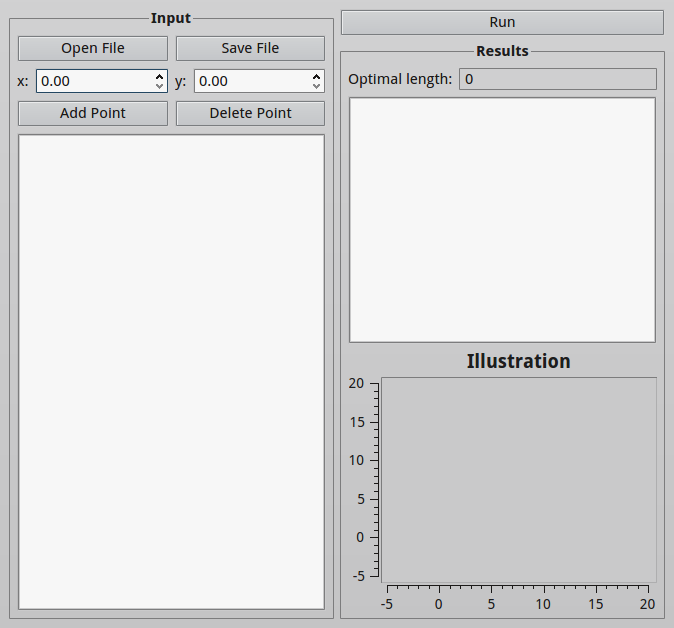
\includegraphics[scale=0.7]{scr.png}
      \caption{Ескіз екранної форми}
      \label{fig:gui}
    \end{figure}

    Користувач може ввести вхідні дані трьома способами:
    \begin{itemize}
      \item Безпосередньо на формі;
      \item З файлу;
      \item Комбінацією двох попередніх способів.
    \end{itemize}

    Після введення даних користувач може зберегти їх до файлу, або використати
    кнопку ,,Run'' для знаходження випуклої оболонки.
    Отриманий результат відображається на координатній площині, а також як
    перелік усіх точок, що є вершинами випуклої оболонки
    (див.~рис.~\ref{fig:final}).

    \begin{figure}[h]
      \centering
      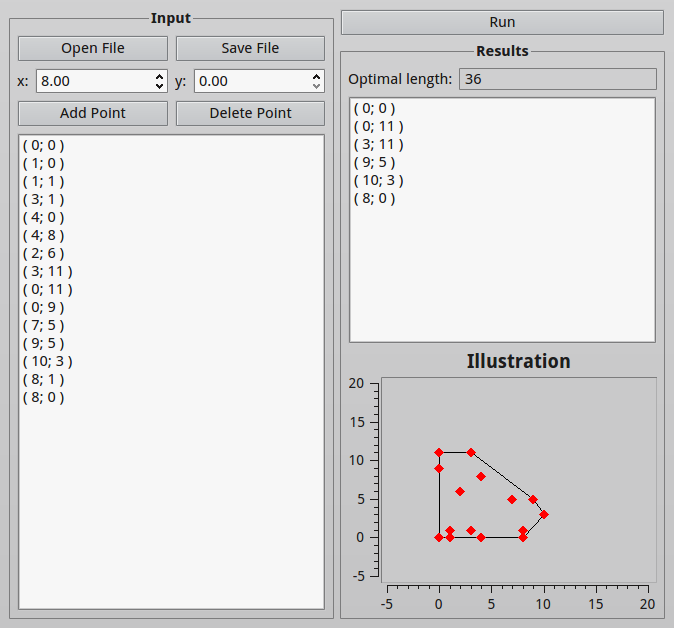
\includegraphics[scale=0.7]{scr1.png}
      \caption{Екранна форма після рішення задачі}
      \label{fig:final}
    \end{figure}

    \clearpage
    \newpage

\section{ВИПРОБУВАННЯ МАТЕМАТИЧНОГО ЗАБЕЗПЕЧЕННЯ}
  При випробуванні математичного забезпечення використовувалися контрольні
  задачі, що були приведені раніш (див. стор.~\pageref{ssec:ex})
  \begin{figure}[h]
    \centering
    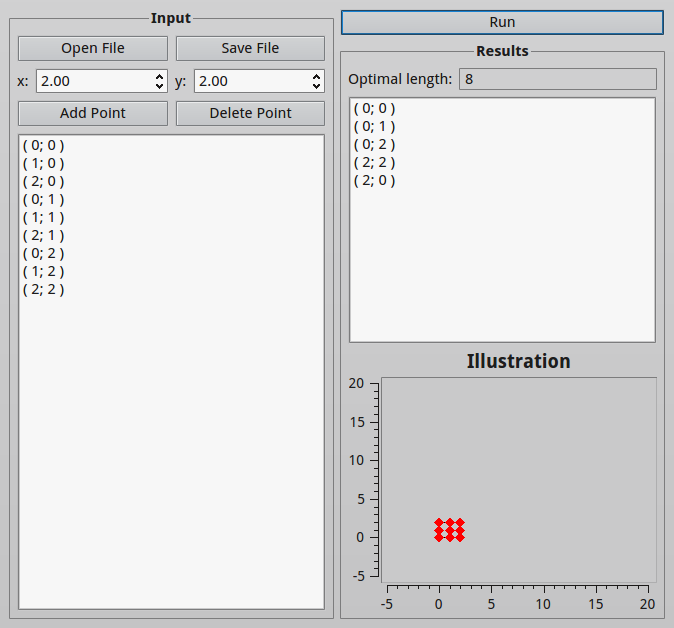
\includegraphics[scale=0.7]{scr2.png}
    \caption{Обчислення прикладу №1}
    \label{fig:ex1}
  \end{figure}

  \begin{figure}[h]
    \centering
    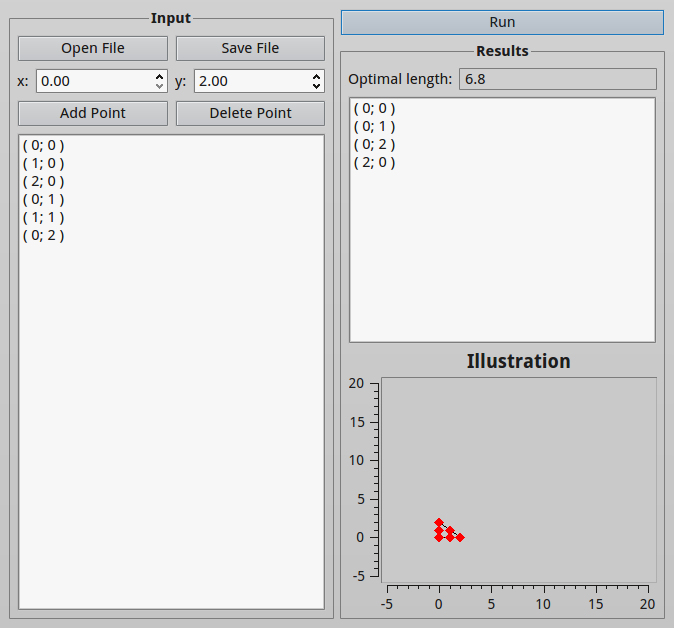
\includegraphics[scale=0.7]{scr3.png}
    \caption{Обчислення прикладу №2}
    \label{fig:ex2}
  \end{figure}

  \clearpage
  \newpage

\section*{ВИСНОВКИ}
\addcontentsline{toc}{section}{ВИСНОВКИ}
  В ході даної роботи було розроблене прикладне програмне забезпечення для
  знаходження випуклої оболонки множини точок на площини за допомогою
  алгоритму (сканування) Грехема.
  Алгоритм Грехема --- простий і ефективний метод пошуку випуклої оболонки,
  що дозволяє побудувати огорожу оптимальної форми, тобто таку, довжина котрої
  буде мінімальною.

  Програмне забезпечення може застосовуватись в багатьох сферах, зокрема при
  планування майбутнього будівництва або при ремонті сучасних інфраструктур.
  Також програма (або бібліотека, розроблена разом з прикладною програмою)
  може бути використана в математичних обрахунках, адже пошук випуклої
  оболонки може бути корисним у багатьох напрямках математичних наук.
  \newpage
    \bibliographystyle{ugost2008ls}
    \renewcommand\bibname{Foo}
    \bibliography{src}
    \newpage
  \ESKDappendix{}{Вихідні тексти\label{sec:app}}
     \subsubsection*{convex\_hull/convex\_hull.hxx}
      \lstinputlisting{afc/convex_hull/convex_hull.hxx}
     \subsubsection*{convex\_hull/convex\_hull.cxx}
      \lstinputlisting{afc/convex_hull/convex_hull.cxx}
     \subsubsection*{convex\_hull/CMakeLists.txt}
      \lstinputlisting{afc/convex_hull/CMakeLists.txt}
     \subsubsection*{cmake/FindQwt6.cmake}
     \lstinputlisting{afc/cmake/FindQwt6.cmake}
     \subsubsection*{CMakeLists.txt}
      \lstinputlisting{afc/CMakeLists.txt}
     \subsubsection*{main\_widget.hxx}
      \lstinputlisting{afc/main_widget.hxx}
      \subsubsection*{main\_widget.cxx}
      \lstinputlisting{afc/main_widget.cxx}
      \subsubsection*{main.cxx}
      \lstinputlisting{afc/main.cxx}
\end{document}
